\documentclass[oneside, 11pt]{article}

\usepackage[T1]{fontenc}
\usepackage[utf8]{inputenc}
\usepackage[english]{babel}

\usepackage{fouriernc}
\usepackage[detect-all, binary-units, separate-uncertainty=true,
            per-mode=symbol, retain-explicit-plus, retain-unity-mantissa=false]{siunitx}

\usepackage{setspace}
\setstretch{1.2}

\setlength{\parskip}{\smallskipamount}
\setlength{\parindent}{0pt}

\usepackage[headheight=14pt]{geometry}
\geometry{marginparwidth=0.5cm, verbose, a4paper, tmargin=3cm, bmargin=3cm,
          lmargin=2cm, rmargin=2cm}

\usepackage{float}

\usepackage[fleqn]{amsmath}
\numberwithin{equation}{section}
\numberwithin{figure}{section}

\usepackage{graphicx}
\graphicspath{{images/}{../../../images/}}

\usepackage{tikz}
\usetikzlibrary{shapes}
\usetikzlibrary{plotmarks}

\newcounter{Exercise}
\setcounter{Exercise}{1}
\usepackage{xcolor}
\definecolor{shadecolor}{gray}{0.9}
\usepackage{framed}
\usepackage{caption}

\usepackage{url}


\usepackage{fancyhdr}
\pagestyle{fancy}
\fancyhf{}
\rhead{\thepage}
\renewcommand{\footrulewidth}{0pt}
\renewcommand{\headrulewidth}{0pt}

\fancypagestyle{firststyle}
{
    \fancyhf{}
    \rhead{\thepage}
    \cfoot{
\includegraphics[height=30pt]{HiSPARClogo}}
    \rfoot{
\includegraphics[height=25pt]{CCbysa}}
    \lfoot{
\includegraphics[height=30pt]{NIKHEFlogo}}
    \renewcommand{\footskip}{50pt}
    \renewcommand{\footrulewidth}{0.1pt}
    \renewcommand{\headrulewidth}{0pt}
}

\newcommand{\figref}[1]{Figuur~\ref{#1}}

\newcommand{\hisparc}{\textsmaller{HiSPARC}\xspace}
\newcommand{\kascade}{\textsmaller{KASCADE}\xspace}
\newcommand{\sapphire}{\textsmaller{SAPPHiRE}\xspace}
\newcommand{\jsparc}{\textsmaller{jSparc}\xspace}
\newcommand{\hdf}{\textsmaller{HDF5}\xspace}
\newcommand{\aires}{\textsmaller{AIRES}\xspace}
\newcommand{\csv}{\textsmaller{CSV}\xspace}
\newcommand{\python}{\textsmaller{PYTHON}\xspace}
\newcommand{\corsika}{\textsmaller{CORSIKA}\xspace}
\newcommand{\labview}{\textsmaller{LabVIEW}\xspace}
\newcommand{\daq}{\textsmaller{DAQ}\xspace}
\newcommand{\adc}{\textsmaller{ADC}\xspace}
\newcommand{\hi}{\textsc{h i}\xspace}
\newcommand{\hii}{\textsc{h ii}\xspace}
\newcommand{\mip}{\textsmaller{MIP}\xspace}
\newcommand{\hisparcii}{\textsmaller{HiSPARC II}\xspace}
\newcommand{\hisparciii}{\textsmaller{HiSPARC III}\xspace}

\DeclareSIUnit{\electronvolt}{\ensuremath{\mathrm{e\!\!\:V}}}

\DeclareSIUnit{\unitsigma}{\ensuremath{\sigma}}
\DeclareSIUnit{\mip}{\textsmaller{MIP}}
\DeclareSIUnit{\adc}{\textsmaller{ADC}}

\DeclareSIUnit{\gauss}{G}
\DeclareSIUnit{\parsec}{pc}
\DeclareSIUnit{\year}{yr}




%document details
\author{N.G. Schultheiss \\ translated and adapted by K. Schadenberg}
\date{}
\title{Michelson \& Morley}


\begin{document}
\maketitle

\section{Introduction}
In 1887 Albert Michelson and Edward Morley tried to measure the relative motion of matter through `luminiferous aether' in what we now call the Michelson-Morley experiment. Their negative results, i.e. no measured difference in the speed of light, led to the dismissal of the then prevalent aether theory and marks the beginnings of what would be the research into special relativity.

You can repeat the Michelson-Morley experiment if you have a Michelson-Morley interferometer at your disposal. In this text we will discuss the results of the 1887 experiment and how this led to the idea of a constant speed of light.

\section{Michelson and Morley}
In the module `Collisions' we explained that collisions which happen at an angle can be analysed by decomposing all movements or momenta into vectors and summing them vectorially. Can we always apply this method? There seem to be no problems when we stick to classical mechanics, i.e. low speeds. But what happens when we go faster and approach the speed of light?

Lets suppose we have a canal exactly 2.5~km long and we are sailing up and down this waterway at exactly 5~km/h. One round trip then takes precisely 1~hour. At one end of the canal is a sluice which is opened to let water flow through the canal at a speed of 0.5~km/h. When going up the canal our boat has to sail against the flow of the water and only reaches a speed of 4.5~km/h relative to the shore. With respect to the water the speed is still 5~km/h. Going down the canal we sail along with the water and now reach a speed of 5.5~km/h relative to the shore. How long does it now take to make one round trip on the canal?

Sailing up the canal now takes a bit longer, 33~minutes and 30~seconds. The trip back is shorter, 26~minutes and 40~seconds. This means the entire journey takes 10~seconds longer because of the flowing water. Knowing this, we can use our sailing time to calculate the velocity of the water. (Naturally you want to verify that no mistakes were made in the calculations, so you might want the check the numbers above.)

In the 19th century the leading opinion amongst scientists was that light is a wave which travels through a certain medium; `aether'. By analogy with a trip on a canal, Michelson and Morley devised an experiment to measure how fast we, on Earth, move through this `aether'. To do this they build an interferometer, see figure~\ref{fig:mm_int}.

\begin{figure}\begin{center}
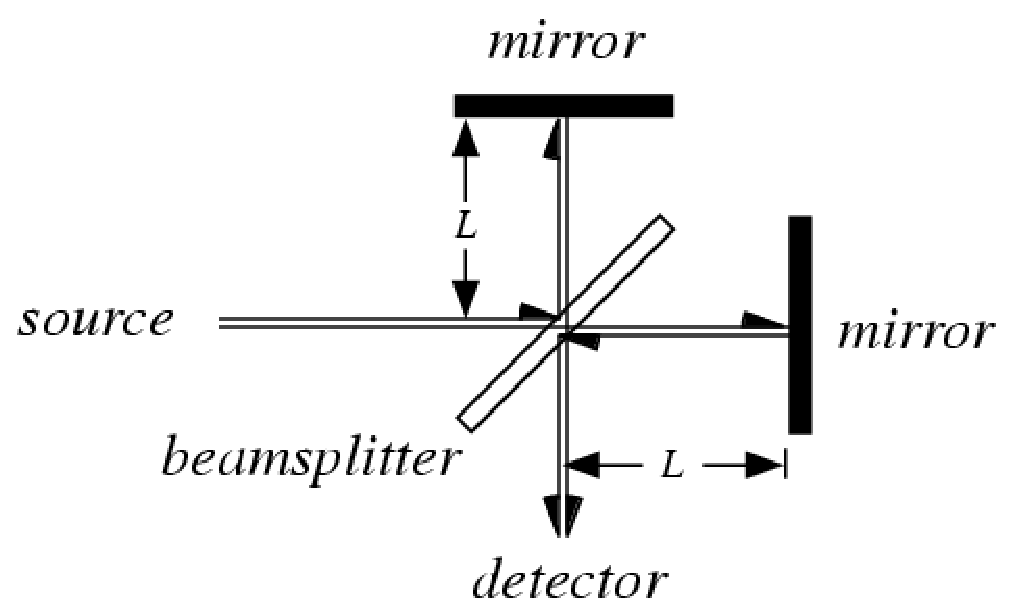
\includegraphics[scale=0.6]{mm_int.eps}
\caption{A Michelson-Morley interferometer. The beam splitter is a 50/50 mirror, it reflects half of the light and lets the other half pass through. The two other mirrors are ordinary mirrors, reflecting all the light.}\label{fig:mm_int}
\end{center}\end{figure}

A pulse of light emitted by the source is split into two separate beams by a beam splitter. The two beams of light follow different paths, but of equal length. One path was directed North to South, the other East to West. The light in the two paths have a different velocity with respect to the aether. The end of both paths is a mirror reflecting the light back to the beam splitter. The two beams are recombined and viewed by a detector. Here the intensity of the light shows whether the light beams are in phase, bright light, or out of phase,  dimmed light. One of the light paths can be changed in length to change how the light beams interfere with each other.

\begin{shaded}
\textbf{Exercise \theExercise \stepcounter{Exercise}} : What type of light source would you use in an interferometer? A naked candle flame, or a candle flame which is being sprayed by table salt?\footnotemark \end{shaded}
\footnotetext{Take a look at the module `Colour' to find out what happens when we introduce table salt into a flame.}

\begin{shaded}
\textbf{Exercise \theExercise \stepcounter{Exercise}} : What is the easiest way to operate the interferometer (or starting position), in or out of phase?\end{shaded}

Michelson and Morley set up their experiment and then turned the entire interferometer. To do this they could just sit and wait because the turning of the Earth around its axis meant that the interferometer was already turning inside the aether. Michelson and Morley expected the see the light intensity change because the light paths where turning inside the aether. Their setup was very sensitive. Even the smallest change, just half a period of the vibration of the light was enough to change from in (bright light) to out of phase (no light).

But the two men saw nothing change. They tried modifying their setup to make it even more sensitive, increasing the path lengths of the light and the number of reflections. But still they saw no change. Turning the light paths into different direction also did not work. They had to conclude that light travels at the same speed in all directions. Simply adding or subtracting the velocity of the medium is no longer a valid way of doing calculations when one is near the speed of light.

\begin{shaded}
\textbf{Exercise \theExercise \stepcounter{Exercise}} : How fast is the Earth moving at the equator due to its rotation? Compare this to the speed of light.\end{shaded}
\begin{shaded}
\textbf{Exercise \theExercise \stepcounter{Exercise}} : The Earth also turn around (orbits) the Sun. Compare the orbital speed of the Earth around the Sun with the speed of light.\end{shaded}
\begin{shaded}
\textbf{Exercise \theExercise \stepcounter{Exercise}} : Estimate the size (the lengths of the light paths) of Michelson and Morley's interferometer needed to detect these changes in velocity.\\
Hint: How many (half or quarter) wavelengths of light do you need? Perhaps take a look at interference in sound.\end{shaded}


\end{document}

